
\documentclass[xcolor=dvipsnames, fontsize=11pt, % Font size
pagesize, % Write page size to dvi or pdf
parskip=half-, t]{beamer}


%
% Choose how your presentation looks.
%
% For more themes, color themes and font themes, see:
% http://deic.uab.es/~iblanes/beamer_gallery/index_by_theme.html
%
\mode<presentation>
  \usetheme{Madrid}      % or try Darmstadt, Madrid, Warsaw, ...
  \usecolortheme{beaver} % or try albatross, beaver, crane, ...
  %\usefonttheme{serif}  % or try serif, structurebold, ...
  \setbeamertemplate{navigation symbols}{}
  \setbeamertemplate{caption}[numbered]
  
\newcounter{example}
\newenvironment<>{exmp}[1][]{%
    \refstepcounter{example}\par\medskip
  \alert{\textbf{Example~\theexample.} }}{}
  
\newenvironment<>{thm}[1][]{%
 \par\medskip
\textbf{\textcolor{MidnightBlue}{\sffamily Theorem.  }}}{}

\newenvironment<>{lem}[1][]{%
	\par\medskip
	\textbf{\textcolor{MidnightBlue}{\sffamily Lemma.  }}}{}

\newenvironment<>{cor}[1][]{%
	\par\medskip
	\textbf{\textcolor{MidnightBlue}{\sffamily Corollary.  }}}{}
\newenvironment<>{exmp*}[1][]{%
\par\medskip
  \alert{\textbf{Example.} }}{}

  
\makeatletter
\newenvironment<>{myproof}[1][\proofname]{%
  \par
  \def\insertproofname{#1.}%
  \pushQED{\qed}
  \textit{\insertproofname}  }
{}
\makeatother

\setbeamertemplate{headline}{}
\setbeamercovered{invisible}

\usepackage{etoolbox}
\makeatletter
\patchcmd{\beamer@continueautobreak}{\frametitle}{\beamer@gobbleoptional}{}{\errmessage{failed to patch}}
\patchcmd{\beamer@continueautobreak}{\framesubtitle}{\beamer@gobbleoptional}{}{\errmessage{failed to patch}}
\makeatother

\makeatother
\setbeamertemplate{footline}
{
  \leavevmode%
  \hbox{%
  \begin{beamercolorbox}[wd=.4\paperwidth,ht=2.25ex,dp=1ex,center]{author in head/foot}%
    \usebeamerfont{author in head/foot}\insertshortauthor
  \end{beamercolorbox}%
  \begin{beamercolorbox}[wd=.6\paperwidth,ht=2.25ex,dp=1ex,center]{title in head/foot}%
    \usebeamerfont{title in head/foot}\insertshorttitle\hspace*{3em}
    \insertframenumber{} / \inserttotalframenumber\hspace*{1ex}
  \end{beamercolorbox}}%
  \vskip0pt%
}
\makeatletter
\setbeamertemplate{navigation symbols}{}

\colorlet{LightSpringGreen}{White!70!SpringGreen}
 \usepackage{transparent}
 \newcommand{\semitransp}[2][35]{\color{fg!#1}#2}
\usepackage[T1]{fontenc}	 % For correct hyphenation and T1 encoding
\usepackage{lmodern} % Default font: latin modern font
%\usepackage{fourier} % Alternative font: utopia
%\usepackage{charter} % Alternative font: low-resolution roman font
\renewcommand{\familydefault}{\sfdefault} % Sans serif - this may need to be commented to see the alternative fonts

\usepackage[english]{babel}
\usepackage[utf8x]{inputenc}

\usepackage{listings}

\lstset
{
    language=[LaTeX]TeX,
    breaklines=true,
    basicstyle=\tt\scriptsize,
    %commentstyle=\color{green}
    keywordstyle=\color{blue},
    %stringstyle=\color{black}
    identifierstyle=\color{magenta},
}


\AtBeginSection[]
{
  \begin{frame}<beamer>
    \frametitle{Outline}
    \tableofcontents[currentsection, hideothersubsections]
  \end{frame}
}



\newcommand{\define}[1]{\textbf{\textcolor{ForestGreen}{#1}}}
\newcommand\kuparrow{\mathbin{\uparrow}}
\usepackage{listings}
\usepackage{setspace}
\definecolor{Code}{rgb}{0,0,0}
\definecolor{Decorators}{rgb}{0.5,0.5,0.5}
\definecolor{Numbers}{rgb}{0.5,0,0}
\definecolor{MatchingBrackets}{rgb}{0.25,0.5,0.5}
\definecolor{Keywords}{rgb}{0,0,1}
\definecolor{self}{rgb}{0,0,0}
\definecolor{Strings}{rgb}{0,0.63,0}
\definecolor{Comments}{rgb}{0,0.63,1}
\definecolor{Backquotes}{rgb}{0,0,0}
\definecolor{Classname}{rgb}{0,0,0}
\definecolor{FunctionName}{rgb}{0,0,0}
\definecolor{Operators}{rgb}{0,0,0}
\definecolor{Background}{rgb}{0.98,0.98,0.98}
\lstdefinelanguage{Python}{
	numbers=left,
	numberstyle=\footnotesize,
	numbersep=1em,
	xleftmargin=1em,
	framextopmargin=2em,
	framexbottommargin=2em,
	showspaces=false,
	showtabs=false,
	showstringspaces=false,
	frame=l,
	tabsize=4,
	% Basic
	basicstyle=\ttfamily\small\setstretch{1},
	backgroundcolor=\color{Background},
	% Comments
	commentstyle=\color{Comments}\slshape,
	% Strings
	stringstyle=\color{Strings},
	morecomment=[s][\color{Strings}]{"""}{"""},
	morecomment=[s][\color{Strings}]{'''}{'''},
	% keywords
	morekeywords={import,from,class,def,for,while,if,is,in,elif,else,not,and,or,print,break,continue,return,True,False,None,access,as,,del,except,exec,finally,global,import,lambda,pass,print,raise,try,assert},
	keywordstyle={\color{Keywords}\bfseries},
	% additional keywords
	morekeywords={[2]@invariant,pylab,numpy,np,scipy},
	keywordstyle={[2]\color{Decorators}\slshape},
	emph={self},
	emphstyle={\color{self}\slshape},
	%
}

\usepackage{import}

\newcommand{\uline}[1]{\rule[0pt]{#1}{0.4pt}}



%------------------------------------------------
% Colors

%------------------------------------------------

%------------------------------------------------
%------------------------------------------------

%------------------------------------------------
% Fonts
\usepackage[T1]{fontenc}	 % For correct hyphenation and T1 encoding
\usepackage{lmodern} % Default font: latin modern font
%\usepackage{fourier} % Alternative font: utopia
%\usepackage{charter} % Alternative font: low-resolution roman font
\renewcommand{\familydefault}{\sfdefault} % Sans serif - this may need to be commented to see the alternative fonts
%------------------------------------------------

%------------------------------------------------
% Various required packages
\usepackage{amsthm} % Required for theorem environments
\usepackage{bm} % Required for bold math symbols (used in the footer of the slides)
\usepackage{graphicx} % Required for including images in figures
\usepackage{tikz} % Required for colored boxes
\usepackage{booktabs} % Required for horizontal rules in tables
\usepackage{multicol} % Required for creating multiple columns in slides
\usepackage{lastpage} % For printing the total number of pages at the bottom of each slide
\usepackage[english]{babel} % Document language - required for customizing section titles
\usepackage{microtype} % Better typography
\usepackage{tocstyle} % Required for customizing the table of contents


%\newtheorem{defi}{Definition}[section]
%\newtheorem{exmp}{Exercise}[section] %Label for examples
\newtheorem{remark}[theorem]{Remark} % Label for remarks
\newtheorem{algorithm}[theorem]{Algorithm} % Label for algorithms
\makeatletter % Correct qed adjustment
%------------------------------------------------

%------------------------------------------------
% The code for the box which can be used to highlight an element of a slide (such as a theorem)
\newcommand*{\mybox}[2]{ % The box takes two arguments: width and content
\par\noindent
\begin{tikzpicture}[mynodestyle/.style={rectangle,draw=Black,thick,inner sep=1.5mm, text justified,top color=white,bottom color=white,above}]\node[mynodestyle,at={(0.5*#1+2mm+0.4pt,0)}]{ % Box formatting
\begin{minipage}[t]{#1}
#2
\end{minipage}
};
\end{tikzpicture}
\par\vspace{-1.3em}}
%------------------------------------------------

%------------------------------------------------
% MODIFICATIONS BY JUSTIN STEVENS
%------------------------------------------------

\usepackage[nodayofweek,level]{datetime}
\usepackage{caption}
\usepackage{subcaption}
\usepackage{hyperref}
\newcommand{\pmid}{\mid\!\mid}
\usepackage{seqsplit}
\usepackage{amsfonts}
\usepackage{float} %use H to force it in place
\usepackage{amssymb} %for nmid
%\usepackage{enumitem} %for itemized lists with stars
\usepackage{amsmath}
\DeclareMathOperator{\lcm}{lcm}
%\usepackage{epigraph}
\usepackage{csquotes}
\usepackage{relsize}
\newcommand{\x}{\color{red}X\color{black}}
%\usepackage[inline]{enumitem}

\makeatletter
% This command ignores the optional argument for itemize and enumerate lists
\newcommand{\inlineitem}[1][]{%
	\ifnum\enit@type=\tw@
	{\descriptionlabel{#1}}
	\hspace{\labelsep}%
	\else
	\ifnum\enit@type=\z@
	\refstepcounter{\@listctr}\fi
	\quad\@itemlabel\hspace{\labelsep}%
	\fi}
\makeatother
\usetikzlibrary{tikzmark}

\usepackage{textcomp}
\newcommand{\ballgolftikz}[1]{%
	\foreach \i  in {0,...,\number\numexpr#1 - 1\relax}{% 
		\pgfmathsetmacro\k{\i*sqrt(3)/1.75}
		\begin{scope}[shift={(\i cm,\k cm)}]
			\foreach \t in {1,...,\number\numexpr 2*#1-1-2*\i\relax}{
				\shade[ball color= gray] (\t,0) circle (.5cm);}
	\end{scope}}
}  
\usepackage{environ}
\usepackage{systeme}
\usepackage{pifont}
\usepackage{marginnote}
\reversemarginpar
\newcommand{\prechili}{\vspace*{1.2em}\hspace*{1.0em}}
\newcommand{\nochili}{\hspace*{3.8em}}
\newcommand{\chili}{\includegraphics[width=1.0em]{images/chili.png}}
\newcommand{\gim}{\marginnote{\chili}}
\newcommand{\yod}{\marginnote{\chili\chili}}
\newcommand{\kurumi}{\marginnote{\chili\chili\chili}}
\newcommand{\pencil}{\prechili\marginnote{\bfseries\ding{48}}}
\newcommand{\defi}{{\bfseries\color{ForestGreen}Definition. }}
\newcommand{\sol}{\textit{Solution.   }}
%\setitemize{label=\usebeamerfont*{itemize item}%
%\usebeamercolor[fg]{itemize item}
%\usebeamertemplate{itemize item}}
\usepackage{mathtools}
\usepackage[symbol, para]{footmisc}
\newenvironment{polyalign}[1][9]
{\array{c*{#1}{@{}>{{}}c<{{}}@{}c@{}}}}
{\endarray}

\usepackage{tabularx}
\usepackage{bm}
\usepackage{mwe}% provides example images (when installed)
\newcommand\measureISpecification{6ex}% not defined in mwe
\newcommand{\ctab}[1]{\raisebox{\dimexpr \measureISpecification/2 -.748ex}{#1}}% vertically centers numbers

\usetikzlibrary{tikzmark}

\usetikzlibrary{arrows} 

\usepgflibrary{fpu}
\usetikzlibrary{positioning}
\usepackage{thmtools}
\theoremstyle{definition}
\declaretheorem[name=\bfseries Problem]{prob}
%\declaretheorem[name=\bfseries Example]{exmp}
\theoremstyle{plain}

\newenvironment{soln}{\begin{myproof}[Solution]}{\end{myproof}}
\newcommand*\circled[1]{\tikz[baseline=(char.base)]{% <---- BEWARE
		\node[shape=circle,draw,inner sep=2pt] (char) {#1};}}
	
\usepackage{comment}
\usepackage{systeme}


\usepackage{scalerel}
\usepackage{stackengine}
\newcommand\showdiv[1]{\overline{\smash{\hstretch{.5}{)}\mkern-3.2mu\hstretch{.5}{)}}#1}}
\newcommand\ph[1]{\textcolor{white}{#1}}


\usepackage{animate}
\usepackage{enumerate}
\setbeamertemplate{title page}
{
  \vbox{}
  \begingroup
    \centering
    {\usebeamercolor[fg]{titlegraphic}\inserttitlegraphic\par}\vskip1em
    \begin{beamercolorbox}[sep=8pt,center]{title}
      \usebeamerfont{title}\inserttitle\par%
      \ifx\insertsubtitle\@empty%
      \else%
        \vskip0.25em%
        {\usebeamerfont{subtitle}\usebeamercolor[fg]{subtitle}\insertsubtitle\par}%
      \fi%
    \end{beamercolorbox}%
    \vskip1em\par
    \begin{beamercolorbox}[sep=8pt,center]{author}
      \insertauthor
    \end{beamercolorbox}
        \vskip1em\par

  \endgroup
  \vfill
}

\usepackage{subcaption}
\usepackage{tabularx}
\usepackage{csquotes}
\usepackage{mathcomp}
\usepackage{xspace}
\usepackage[normalem]{ulem}
\usepackage{cancel}

\def\stacktype{L}
\def\useanchorwidth{T}

\renewcommand\xcancel[1]{\bcancel{\cancel{#1}}}
\renewcommand\bcancel[1]{\stackon[7pt]{#1}{\rotatebox{-30}{\rule{2.9ex}{1pt}}}}
\renewcommand\cancel[1]{\stackon[0pt]{#1}{\rotatebox{30}{\rule{2.9ex}{1pt}}}}
\newcommand\strike[1]{\stackon[3.3pt]{#1}{\rule{2.9ex}{1pt}}}
\newcommand\vstrike[1]{\stackon{#1}{\smash{\rule[-3pt]{1pt}{2.9ex}}}}

\makeatletter
\def\th@mystyle{
	\itshape % body font
	\setbeamercolor{block title example}{bg=orange,fg=white}
	\setbeamercolor{block body example}{bg=orange!20,fg=black}
	\def\inserttheoremblockenv{exampleblock}
}
\makeatother
\theoremstyle{mystyle}
\newtheorem*{lemma2}{Lemma}
\usepackage{tabulary}
\usepackage{etoolbox}
\usepackage{xcolor,colortbl}
\usepackage{multicol}
\usepackage{listings}
\titlegraphic{
\includegraphics[height=0.09\textwidth]{uofa.png}}
\title[Artificial Intelligence for Beginners]{Gradient Descent}
\subtitle{Towards Neural Networks}
\newcommand{\norm}[1]{\left\lVert#1\right\rVert}
\author[Justin Stevens]{\large Justin Stevens \\ \large Undergraduate AI Society \\  April 2nd, 2019} % 
\date{}
\setbeamertemplate{button}{\tikz
	\node[
	inner xsep=10pt,
	draw=structure!80,
	fill=structure!50,
	rounded corners=4pt]  {\large\insertbuttontext};}
\usepackage{asymptote}
\usepackage{animate}
\usepackage{xmpmulti}
\begin{document}
	\renewcommand{\thefootnote}{\fnsymbol{footnote}}
	\begin{frame}[c]
	\centering
	\titlepage
\end{frame}
\section{Decision Making}
\subsection{Perceptrons}
\begin{frame}{Should I Stay or Should I Go?}
Let's say I'm deciding on a given day whether or not to go to  an Edmonton Oilers game. Here are the factors that will influence my decision: \pause 
\begin{itemize}
\item Are the tickets cheap or expensive?
\item Do I have the time to go?
\item Do I care about the team they're playing?
\end{itemize} \pause 
We'll make my decision by encoding each possible input as a vector $\bar{\bold{x}}$: \pause
\begin{table} \center 
\begin{tabular}{ccc|c}
Ticket Prices & Availability & Interest & $\bar{\bold{x}}$\\ \hline 
Cheap & Yes & Yes & $(1,1,1)$ \\
Cheap & No & No & $(1,0,0)$ \\
Cheap & Yes & No & $(1,1,0)$ \\
Cheap & No & Yes & $(1,0,1)$  \\
Expensive & Yes & Yes & $(0,1,1)$ \\
Expensive & No & No & $(0,0,0)$ \\
Expensive & No & Yes & $(0,0,1)$ \\
Expensive & Yes & No & $(0,1,0)$ 
\end{tabular}
\end{table}
\end{frame}

\begin{frame}{How Will I Make my Decision?}
Let's say I don't care much about price, but I do care about my availability and interest. In this case, the corresponding weights might be $\bar{\bold{w}}=(1, 6, 3)$. \pause We can then compute the dot product $\bar{\bold{w}}\cdot \bar{\bold{x}}$ for each possible input:  
\begin{table} 
\center 
\begin{tabular}{cccc|c}
Ticket Prices & Availability & Interest & $\bar{\bold{x}}$ & $\bar{\bold{w}}\cdot \bar{\bold{x}}$ \\ \hline 
Cheap & Yes & Yes & $(1,1,1)$ & $10$ \\
Cheap & No & No & $(1,0,0)$ & $1$ \\
Cheap & Yes & No & $(1,1,0)$ & $7$\\
Cheap & No & Yes & $(1,0,1)$ & $4$   \\
Expensive & Yes & Yes & $(0,1,1)$ & $9$ \\
Expensive & No & No & $(0,0,0)$  & $0$ \\
Expensive & No & Yes & $(0,0,1)$ & $3$\\
Expensive & Yes & No & $(0,1,0)$ & $6$
\end{tabular}
\end{table} \pause
\vspace{0.05\textheight}
We can now define my \textbf{activation threshold}, $t$, which will determine whether or not I go to the game, represented in binary.
\end{frame}

\begin{frame}{Formula for Decision Making}
The general formula for my decision to go to the Oilers game is $$\text{output}=\begin{cases} 0 & \text{ if } \bar{\bold{w}}\cdot \bar{\bold{x}}<t \\ 
1 & \text{ if } \bar{\bold{w}}\cdot \bar{\bold{x}}\ge t. \end{cases}$$ \pause 
For instance, if $t=9$, we see I'll only go if I'm both available and interested. \pause If $t=7$, I'll also go if the tickets are cheap and I'm available:
\begin{table} 
\center 
\begin{tabular}{cccc|c}
Ticket Prices & Availability & Interest & $\bar{\bold{x}}$ & $\bar{\bold{x}}\cdot \bar{\bold{w}}$ \\ \hline 
\textbf{\textcolor{Green}{Cheap}} & \textbf{\textcolor{Green}{Yes}} & \textbf{\textcolor{Green}{Yes}} & $(1,1,1)$ & \textbf{\textcolor{Green}{10}} \\
Cheap & No & No & $(1,0,0)$ & $1$ \\
\textbf{\textcolor{Green}{Cheap }}& \textbf{\textcolor{Green}{Yes }}& \textbf{\textcolor{Green}{No}} & $(1,1,0)$ & \textbf{\textcolor{Green}{7}} \\
Cheap & No & Yes & $(1,0,1)$ & $4$   \\
\textbf{\textcolor{Green}{Expensive}} & \textbf{\textcolor{Green}{Yes}} & \textbf{\textcolor{Green}{Yes}} & $(0,1,1)$ & \textbf{\textcolor{Green}{9}} \\
Expensive & No & No & $(0,0,0)$  & $0$ \\
Expensive & No & Yes & $(0,0,1)$ & $3$\\
Expensive & Yes & No & $(0,1,0)$ & $6$
\end{tabular}
\end{table}
\end{frame}
\begin{frame}{Perceptrons}
This is a simplified model of a \textbf{perceptron}. The idea was developed by Frank Rosenblatt at Cornell in 1957, and is often used in psychology. \pause 

\begin{figure}
\center
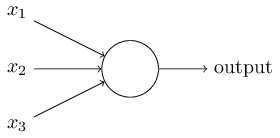
\includegraphics[scale=0.66]{perc.png}
\caption{\textit{Source: Nielsen}}
\end{figure} \pause
\vspace{0.05\textheight} 
Each of these lines collect evidence and are weighted to produce an output. \pause In practice, our inputs and outputs don't necessarily have to be binary; they can be real-valued. We therefore have to define a new activation function.
\end{frame}
\subsection{Activation Functions}
\begin{frame}[c]{Introducing the Bias}
Instead of comparing our weighted sum to a threshold, we instead \textit{add} a bias, $b$, to our weighted sum. We write this as $\bar{\bold{w}}\cdot \bar{\bold{x}}+b$ instead. \pause Then $$\text{output}=\begin{cases} 0 & \text{ if } \bar{\bold{w}}\cdot \bar{\bold{x}}+b<0 \\ 
1 & \text{ if } \bar{\bold{w}}\cdot \bar{\bold{x}}+b\ge 0. \end{cases}$$
This is known as the \textit{heaviside step function}. We'll extend our model to multiple outputs soon, but first we'll examine other activation functions. \pause
\begin{figure}
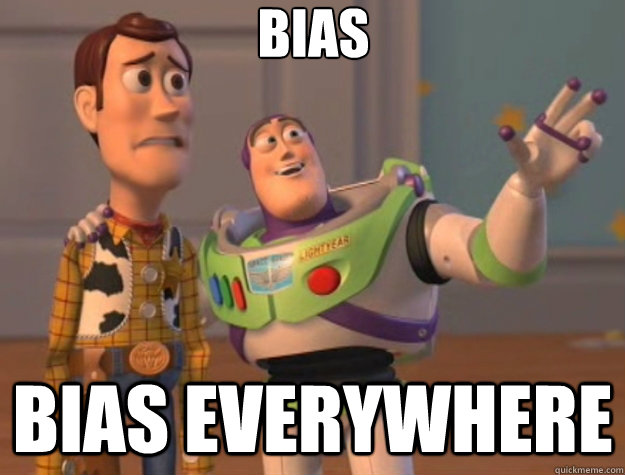
\includegraphics[scale=0.23]{bias.jpg} 
\end{figure}
\end{frame}
\begin{frame}{Rectified Linear Unit}
If we want our outputs to be non-negative, we use the \textbf{rectified linear unit}, $$f(x)=\text{max}\{0, x\}.$$ \pause Graphically, we can see:
\begin{figure}
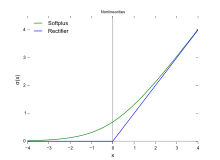
\includegraphics[scale=0.18]{rectifier.png}
\caption{Rectifier, and a smooth approximation $\log(1+e^x)$. (\textit{Source: Wikipedia}).}
\end{figure}

\end{frame}

\begin{frame}{Sigmoid Function} 
As we saw above, our output doesn't necessarily have to be a $0$ or $1$; using a rectified linear unit, it can be any non-negative number.  However, for computational purposes, it's easiest if our outputs live in the range $(0,1)$. \pause We now define the \textbf{sigmoid} or logistic function, $\sigma(z)=\frac{1}{1+e^{-z}}$. \pause Graphically,
\begin{figure}
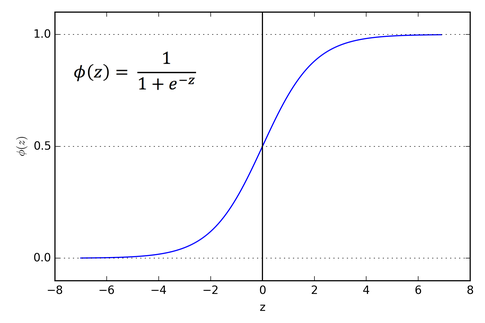
\includegraphics[scale=0.36]{logistic.png}
\caption{As $z\to \infty$, we see $\sigma(z)\to 1$. Alternatively, as $z\to -\infty$, $\sigma(z)\to 0$. (\textit{Source: Towards Data Science}).}
\end{figure}
\end{frame}




\section{Classifying Digits through MNIST}
\subsection{Defining the Problem}
\begin{frame}[c]{Example Images}
In \textbf{supervised learning} problems, we're given a set of training data with labels, which we try to learn. We'll use a generalization of the perceptron with different neurons, for which we try to learn the best possible weights. \pause 
\begin{figure} 
\center
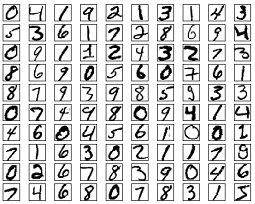
\includegraphics{mnist_100_digits.png}
\caption{How would you devise a system for a \textbf{computer} to classify the digits? How can we best utilize the data set, known as MNIST?  (\textit{Source: Nielsen}) }
\end{figure}
\end{frame}

\begin{frame}[c]{MNIST Dataset}
\begin{itemize}
\item The MNIST database contains seventy thousand handwritten digits.  \pause 
\begin{itemize}
\item Each data-point contains both an image, and the desired digit.
\item $60,000$ images are designated for training, and $10,000$ for testing:
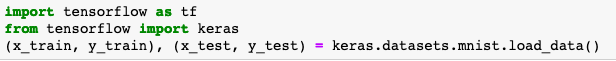
\includegraphics[scale=0.42]{load.png}
\end{itemize} \pause 
\item Each image contains pixels ranging $0$ to $255$, in decreasing darkness. \pause
\item  An individual image is a $28\times 28$ array of pixels.\pause  
\item The desired digit is represented as a number from $0$ to $9$. \pause 
\end{itemize}
We'll build a model from the training images that will learn to classify digits!
\end{frame}
\subsection{Neural Networks}
\begin{frame}{What we're building towards}
\begin{figure}
\center
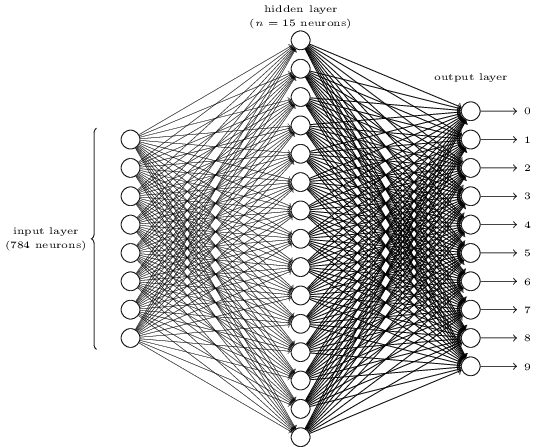
\includegraphics[scale=0.36]{goal.png}
\caption{A simple neural network structure. The input vectors on the left hand side have $28\times 28=784$ inputs for each pixel, and the output layer has $10$ digits. (\textit{Source: Nielsen}) }
\end{figure}
\end{frame}
\subsection{Randomizing Weights and Biases}
\begin{frame}{Extending our Model}
All of our weights and bias will be initialized from a normal distribution with mean $0$ and standard deviation $1$. 
\begin{figure}
\center
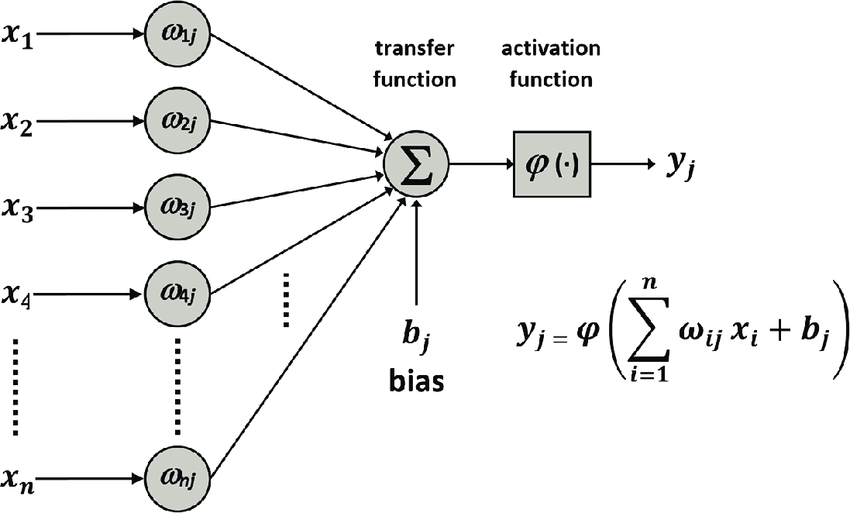
\includegraphics[scale=0.28]{perceptron.png}
\caption{\textit{Source: Daniel Alvarez, InTech}}
\end{figure}
\end{frame}
\begin{frame}{Hidden Layer}
The role of the \textbf{hidden layer} is to hold intermediate calculations. These will in turn be used to compute the output layer. To produce the hidden layer, we must have an $784\times 15$ weight matrix, as seen below: $$W=\begin{pmatrix} w_{11} & w_{12}  & \cdots &  w_{1,784} \\  w_{21} & w_{22} & \cdots & w_{2,784} \\  \vdots & \vdots  & \ddots & \vdots \\  w_{15, 1} & w_{15, 2}  & \cdots & w_{15, 784} \end{pmatrix}, \quad \bold{x}=\begin{pmatrix} x_1 \\ x_2 \\ \vdots  \\ \vdots \\ x_{784} \end{pmatrix}, \quad \bold{b}=\begin{pmatrix} b_1 \\ b_2 \\ \vdots \\ b_{15} \end{pmatrix}.$$
We take the dot product of each \textbf{row} with our input vector $\bold{x}$. We then add our bias vector, $\bold{b}$, which is $15\times 1$. We finally apply our activation: $$\bold{h}=\sigma(W\bold{x}+\bold{b}).$$
Notice the sigmoid function is applied component wise.
\end{frame}
\subsection{Softmax and One-Hot Encoding}
\begin{frame}{Output Layer}
We must now define a transformation from $\mathbb{R}^{15}$ to $\mathbb{R}^{10}$, which we can do using a $10\times 15$ weight matrix $\hat{W}$. We can then add a $10\times 1$ bias vector, $\hat{\bold{b}}$. \pause We can write this as $\bold{f}=\begin{pmatrix} \hat{w}_{11} & \hat{w}_{12} & \cdots & \hat{w}_{1,15} \\ \hat{w}_{21} & \hat{w}_{22} & \cdots & \hat{w}_{2,15} \\ \vdots & \vdots & \vdots & \vdots \\ \hat{w}_{10,1} & \hat{w}_{10,2} & \cdots & \hat{w}_{10,15} \end{pmatrix}\begin{pmatrix} h_{1} \\ h_2 \\ \vdots \\ \vdots \\ h_{15} \end{pmatrix}+\begin{pmatrix} \hat{b}_{1} \\ \hat{b}_2 \\ \vdots \\ \hat{b}_{10} \end{pmatrix}$. \pause We aren't done yet! We want the output to be the probability an image is a specific digit. To do so, we use a \textbf{softmax} activation. The formula is $$\displaystyle \text{softmax}\left(\bold{z}\right)_{j}=\frac{e^{z_j}}{\sum_{k=1}^{10}e^{z_k}}, \quad 1\le j \le 10.$$ Notice the sum of these values will always be $1$. \pause The full computation is $$\bold{f}=\hat{W}\bold{h}+\bold{b}, \quad \bold{o}=\text{softmax}\left(\bold{f}\right).$$  
% For instance, $\text{softmax}(\begin{pmatrix} 4 \\ 2 \\ 1   \end{pmatrix})=\begin{pmatrix} 0.8438 \\ 0.1142 \\ 0.0420 \end{pmatrix}$ has max probability $84.38\%$.
  \end{frame}
  \begin{frame}{One Hot Encoding}
Once we've computed the output, we need a way to compare it to our desired result. However, $\bold{o}$ is a $10\times 1$ vector, whereas our desired digit $y_{\text{train}}(\bold{x})$ is a scalar. We therefore encode the digit as a $10\times 1$ vector:  \pause
\begin{table}
  \center \begin{tabular}{ccccc}
  $\begin{pmatrix} 1 \\ 0 \\ 0 \\ \vdots \\ 0 \end{pmatrix}$ & $\begin{pmatrix} 0 \\ 1 \\ 0 \\ \vdots \\ 0 \end{pmatrix}$ & $\begin{pmatrix} 0 \\ 0 \\ 1 \\ \vdots \\ 0 \end{pmatrix}$ & $\cdots$ & $\begin{pmatrix} 0 \\ 0 \\ 0 \\ \vdots \\ 1 \end{pmatrix}$ \\ \hline $0$ & $1$ & $2$ & $\cdots$ & $9$
  \end{tabular}  
  \end{table}
  \vspace{0.025\textheight}
  \pause
 The code for this is relatively simple: 
 \begin{figure}[H] \center 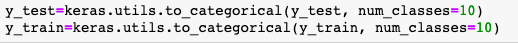
\includegraphics[scale=0.54]{onehot.png} \end{figure}

 \end{frame}
 \subsection{Loss Function}
 \begin{frame}{Negative Log Likelihood}
 To compute how accurate our model was at predicting a given value, we need a \textbf{loss} function. In this case, it's easiest to use \textit{negative log likelihood}.  \pause
 \begin{figure}[H] \center 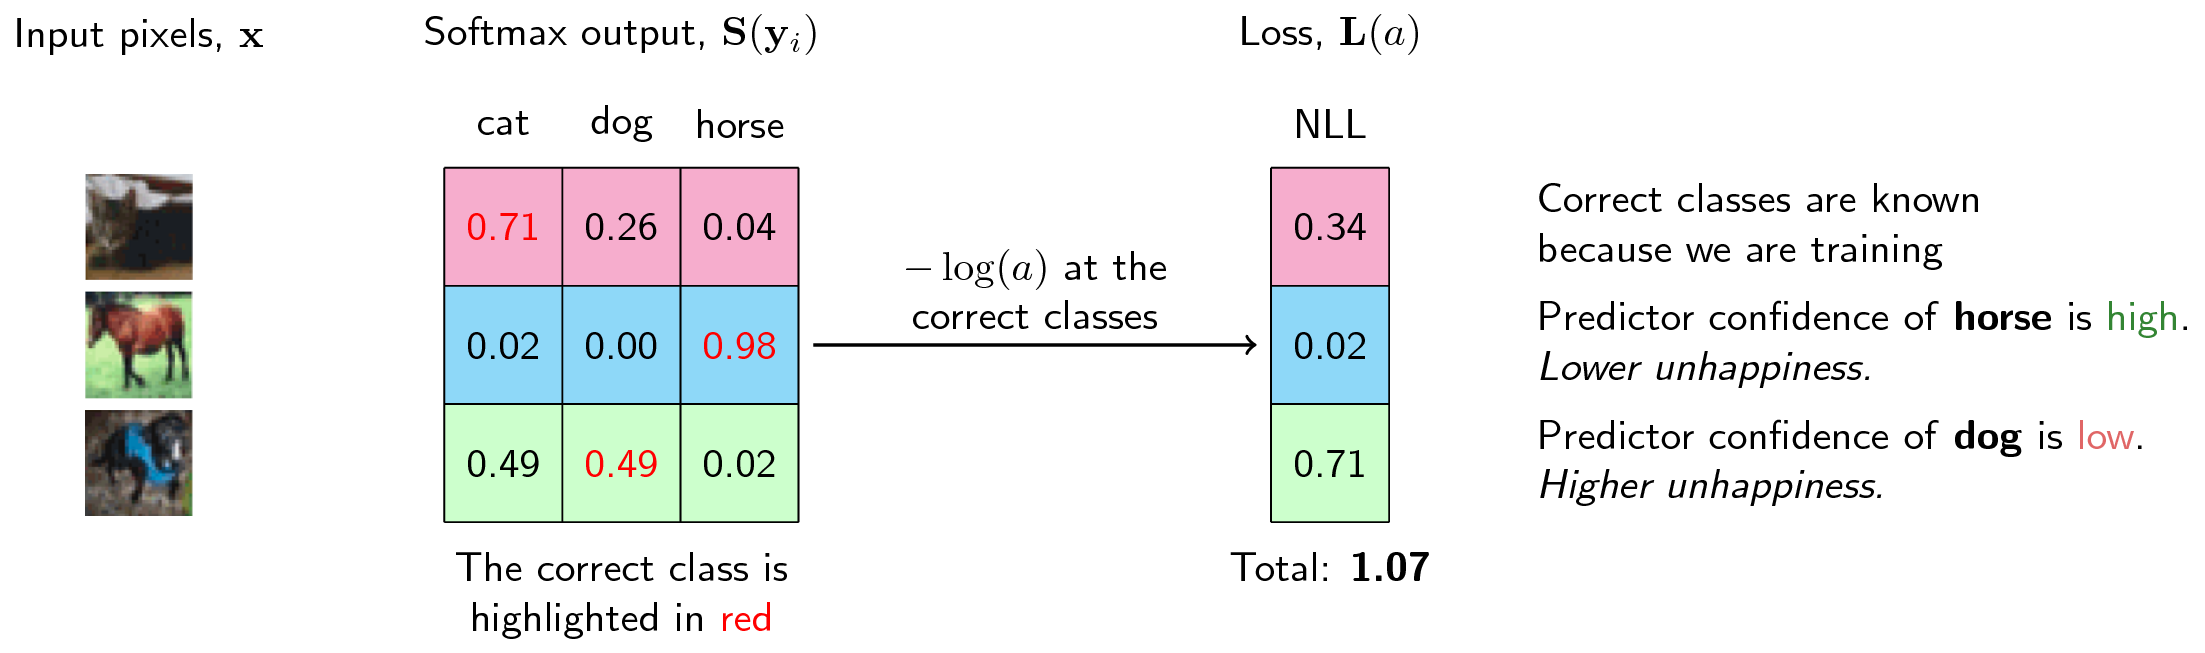
\includegraphics[scale=0.15]{neg_log_demo.png}
 \caption{\textit{Source: LJ Mirand}} \end{figure} \pause 
To compute the loss for an individual training example, $\bold{x}$, with one-hot encoded label $y_{\text{train}}(\bold{x})$, and output $\bold{o}$, we compute $$L(\bold{x})=-y_{\text{train}}(\bold{x})\cdot \log \bold{o}=-\log(o_j),$$ where $j$ is the true label.
 \end{frame}
 \begin{frame}{Graph of Negative Log}
Recall $L(\bold{x})=-\log(o_j)$. Since $o_j$ is between $0$ and $1$, we can graph the function, noting it approaches $0$ as $o_j\to 1$, and goes to $\infty$ as $o_j\to 0$.
\begin{figure}[H] \center 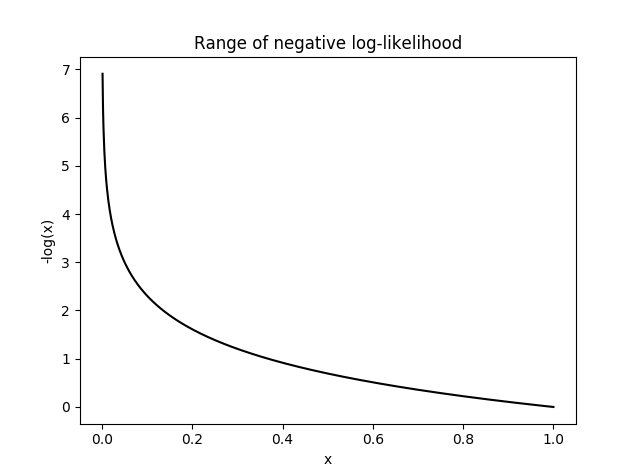
\includegraphics[scale=0.45]{neg_log.png}
\caption{\textit{Source:  LJ Mirand}}\end{figure}
 \end{frame}
 \begin{frame}{Summarizing the Loss Function}
 \begin{figure}[H] \center 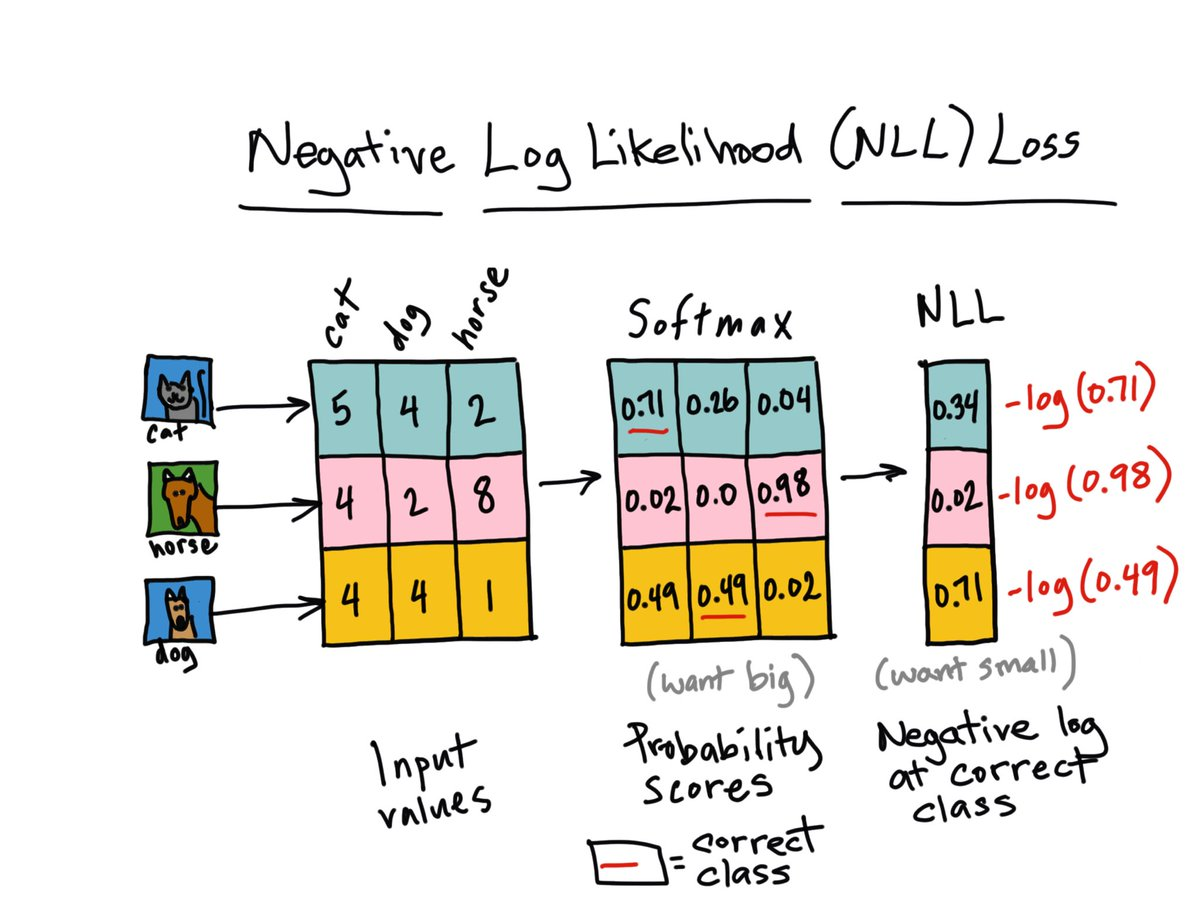
\includegraphics[scale=0.18]{fullpic.jpg}
 \caption{\textit{Source: Micheleen Harris}}
 \end{figure}
 \end{frame}
 \subsection{Gradient Descent}
 \begin{frame}{Gradient Descent Intuition}
Our goal is to minimize loss with respect to weights and biases. To simplify the model, let's assume $C$ is a function of two variables: $v_1$ and $v_2$. 
\begin{figure}
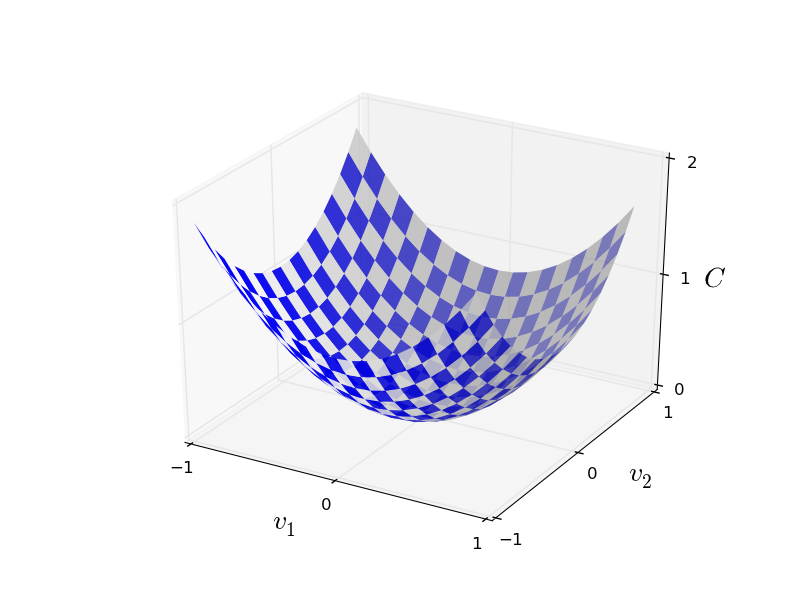
\includegraphics[scale=0.36]{valley.png}
\caption{\textit{Source: Nielsen}}
\end{figure}
 \end{frame}
 \begin{frame}{Gradient Descent II}
 We see how much $C$ changes as we nudge $v_1$ and $v_2$. Approximating, $$\Delta C\approx \frac{\partial C}{\partial v_1}\Delta v_1+\frac{\partial C}{\partial v_2}\Delta v_2.$$ \pause We  find the optimal way to adjust $\Delta v_1$ and $\Delta v_2$ so that $\Delta C$ is negative. We define $\Delta v=\binom{\Delta v_1}{\Delta v_2}$ and the \textbf{gradient} vector $\nabla C=\begin{pmatrix} \frac{\partial C}{\partial v_1} & \frac{\partial C}{\partial v_2} \end{pmatrix}^{T}.$\pause 
 Therefore, $$\Delta C\approx \nabla C\cdot \Delta v.$$ \pause By the Cauchy-Schwartz inequality, the direction of greatest descent is $\Delta v=-\lambda \nabla C$. In this case, $\Delta C\approx \nabla C\cdot -\lambda \nabla C=-\lambda \norm{\nabla C}^2\ll 0$. \pause 
 
 \vspace{0.04\textheight}
 We therefore update $v\to v'=v-\lambda \nabla C$, where $\lambda$ is the \textbf{learning rate}. \pause
 
We iterate this process in the hopes of finding a local minimum of $C$. This process can fairly easily generalize from $2$ variables to $n$ variables if we wish. 
 \end{frame}
 \begin{frame}[c]{Gradient Descent III}
 \begin{figure}[H] \center
 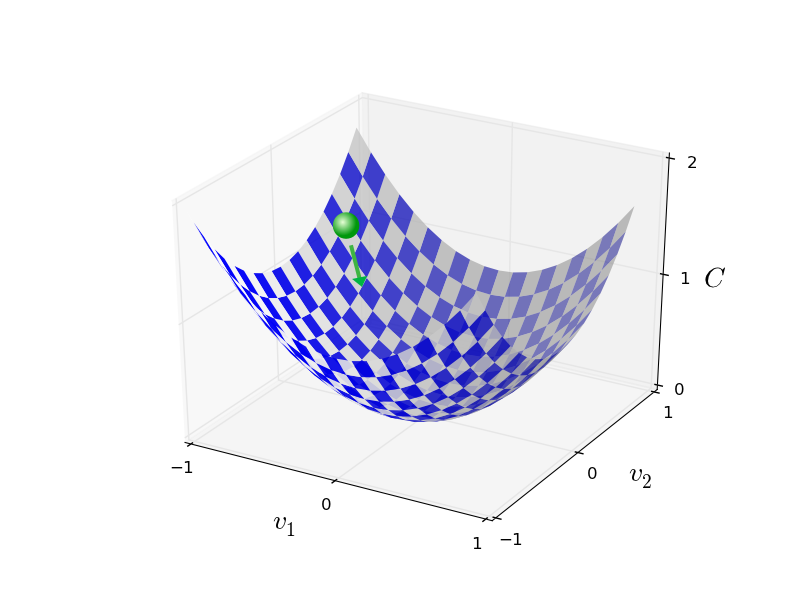
\includegraphics[scale=0.32]{valley_with_ball.png}
 \caption{\textit{Source: Nielsen}}
 \end{figure}
 
 \end{frame}
 \subsection{Backpropagation}
  \begin{frame}{Backpropagation Part I}
In our hidden layer, we have $784\times 15+15\times 1=11,775$ weights and biases to train on. In the output layer, we only have $15\times 10+10\times 1=160$. \pause We'll answer the question: how much does our loss function depend on these parameters?  To answer this, we need the chain rule from calculus: \pause

$$L=-\log \left(o_j\right), \quad o_j=\frac{e^{f_j}}{e^{f_1}+e^{f_2}+\cdots+e^{f_{10}}}.$$
Then $\frac{\partial L}{\partial f_j}=\frac{\partial L}{\partial o_j}\frac{\partial o_j}{\partial f_j}=-\frac{1}{o_j}\frac{\partial o_j}{\partial f_j}$. Using the quotient rule and some algebra, \pause \begin{align*} \frac{\partial L}{\partial f_j}&=-\frac{1}{o_j}\frac{\left(e^{f_1}+\cdots+e^{f_{10}}\right)e^{f_j}-e^{f_j}e^{f_j}}{\left(e^{f_1}+\cdots+e^{f_{10}}\right)^2} \\ &=-\frac{e^{f_1}+\cdots+e^{f_{10}}}{e^{f_j}}\cdot \frac{e^{f_j}\left(e^{f_1}+e^{f_2}+\cdots+e^{f_{10}}-e^{f_j}\right)}{\left(e^{f_1}+\cdots+e^{f_{10}}\right)^2} \\ &=-\frac{e^{f_1}+\cdots+e^{f_{10}}-e^{f_j}}{e^{f_1}+\cdots+e^{f_{10}}}=-\left(1-o_j\right)=o_j-1. \end{align*}

  \end{frame}
  \begin{frame}{Backpropagation Part II}
$$L=-\log \left(o_j\right), \quad o_j=\frac{e^{f_j}}{e^{f_1}+e^{f_2}+\cdots+e^{f_{10}}}.$$ \pause  If $i\neq j$, by the chain rule $\frac{\partial L}{\partial f_i}=\frac{\partial L}{\partial o_j}\frac{\partial o_j}{\partial f_i}=-\frac{1}{o_j}\frac{\partial o_j}{\partial f_i}.$ \pause Using the quotient rule, \begin{align*} \frac{\partial L}{\partial f_i} &=-\frac{1}{o_j}\cdot \frac{-e^{f_j}e^{f_i}}{\left(e^{f_1}+e^{f_2}+\cdots+e^{f_{10}}\right)^2} \\ &=\frac{e^{f_1}+e^{f_2}+\cdots+e^{f_{10}}}{e^{f_j}}\cdot \frac{e^{f_j}e^{f_i}}{\left(e^{f_1}+e^{f_2}+\cdots+e^{f_{10}}\right)^2} \\ &=\frac{e^{f_i}}{e^{f_1}+\cdots+e^{f_{10}}}=o_i. \end{align*} \pause
We've now computed how much our loss function depends upon the final activations before applying the softmax.  We now go back a layer and see how much $L$ depends upon $\hat{W}$ and $\hat{b}$, and store these results in a gradient.
\end{frame}
\begin{frame}{Backpropagation Part III}
We can write this as $\bold{f}=\begin{pmatrix} \hat{w}_{11} & \hat{w}_{12} & \cdots & \hat{w}_{1,15} \\ \hat{w}_{21} & \hat{w}_{22} & \cdots & \hat{w}_{2,15} \\ \vdots & \vdots & \vdots & \vdots \\ \hat{w}_{10,1} & \hat{w}_{10,2} & \cdots & \hat{w}_{10,15} \end{pmatrix}\begin{pmatrix} h_{1} \\ h_2 \\ \vdots \\ \vdots \\ h_{15} \end{pmatrix}+\begin{pmatrix} \hat{b}_{1} \\ \hat{b}_2 \\ \vdots \\ \hat{b}_{10} \end{pmatrix}$. \vspace{0.025\textheight} \pause 

By matrix multiplication, $f_k=\hat{w}_{k1}h_1+\hat{w}_{k2}h_2+\cdots+\hat{w}_{k,15}h_{15}+b_k$. \pause Therefore, $\displaystyle \frac{\partial L}{\partial \hat{w}_{k\ell}}=\sum_{i=i}^{10} \frac{\partial L}{\partial f_i}\frac{\partial f_i}{\partial \hat{w}_{k\ell }}=\frac{\partial L}{\partial f_k}\frac{\partial f_k}{\partial \hat{w}_{k\ell}}=\begin{cases} o_km_{\ell} & \text{ if } k\neq j \\ 
\left(o_k-1\right)m_{\ell} & \text{ if } k=j \end{cases}$. \pause We can similarly see that $\displaystyle \frac{\partial L}{\partial b_k}=\sum_{i=1}^{10} \frac{\partial L}{\partial f_i}\frac{\partial f_i}{\partial b_k}=\begin{cases} o_k & \text{ if } k\neq j \\ o_k-1&  \text{ if } k=j. \end{cases}$. \pause \vspace{0.025\textheight}

We store these results as the first $160$ entries in a gradient $\nabla L$. The key idea of back-propagation is we continually \textbf{propagate the error backwards} through the neural network, adding new terms as we go.

\end{frame}


\subsection{References}
\begin{frame}[c]{References}
\setbeamertemplate{itemize items}[triangle]

\href{http://neuralnetworksanddeeplearning.com/chap1.html}{\beamergotobutton{Michael Nielsen: Using neural nets to recognize handwritten digits}} \smallskip

\href{https://ljvmiranda921.github.io/notebook/2017/08/13/softmax-and-the-negative-log-likelihood/}{\beamergotobutton{LJ Mirand: Understanding softmax and the negative log-likelihood}} \smallskip

\href{https://towardsdatascience.com/a-beginners-guide-to-neural-networks-part-two-bd503514c71a}{\beamergotobutton{Towards Data Science: A Beginner's Guide to Neural Networks}} \medskip





\href{http://scs.ryerson.ca/~aharley/vis/fc/}{\beamergotobutton{3d Visualizing a Neural Network}} \smallskip


\end{frame}
\end{document}